\chapter{Control Design and Development}



\section{Static Controller} \label{NeuralController}

The development of the controller, inspired by the methodologies proposed in the paper \cite{QSC}, aims to determine the optimal muscle excitation to stabilize the wrist's position. The architectural layout of this controller is portrayed on Figure \ref{fig:BDC}.

The input of the controller is the desired arm configuration. Using the Inverse of the Arm Statics model, described in Section \ref{sec:model}, the required torques to maintain the arm in a static position are computed. These torques are subsequently given as an input into the Muscle Torque Production model, elaborated in Section \ref{sec:model}. This model outputs the corresponding muscle excitations which will define the neural excitation input for the Dynamic Arm Simulator. 

The Dynamic Arm Simulator will then determine the arm's dynamics in accordance with the Rosenbrock equation, as explained in Section \ref{sec:dynamics}. Post these dynamic computations, the wrist's actual position is deduced. The error between the desired and the actual wrist position will drive a PID Controller, which will calculate the corrective force needed to match the desired wrist position. The kinematic Jacobian, Section \ref{sec:torque}, will compute the requisite corrective torque. This torque, when combined with the desired torque from the Inverse Arm Statics, provides the total torque which is then input to the Inverse Muscle Torque model, closing the control loop. 


\begin{figure}[h!]
    \centering
    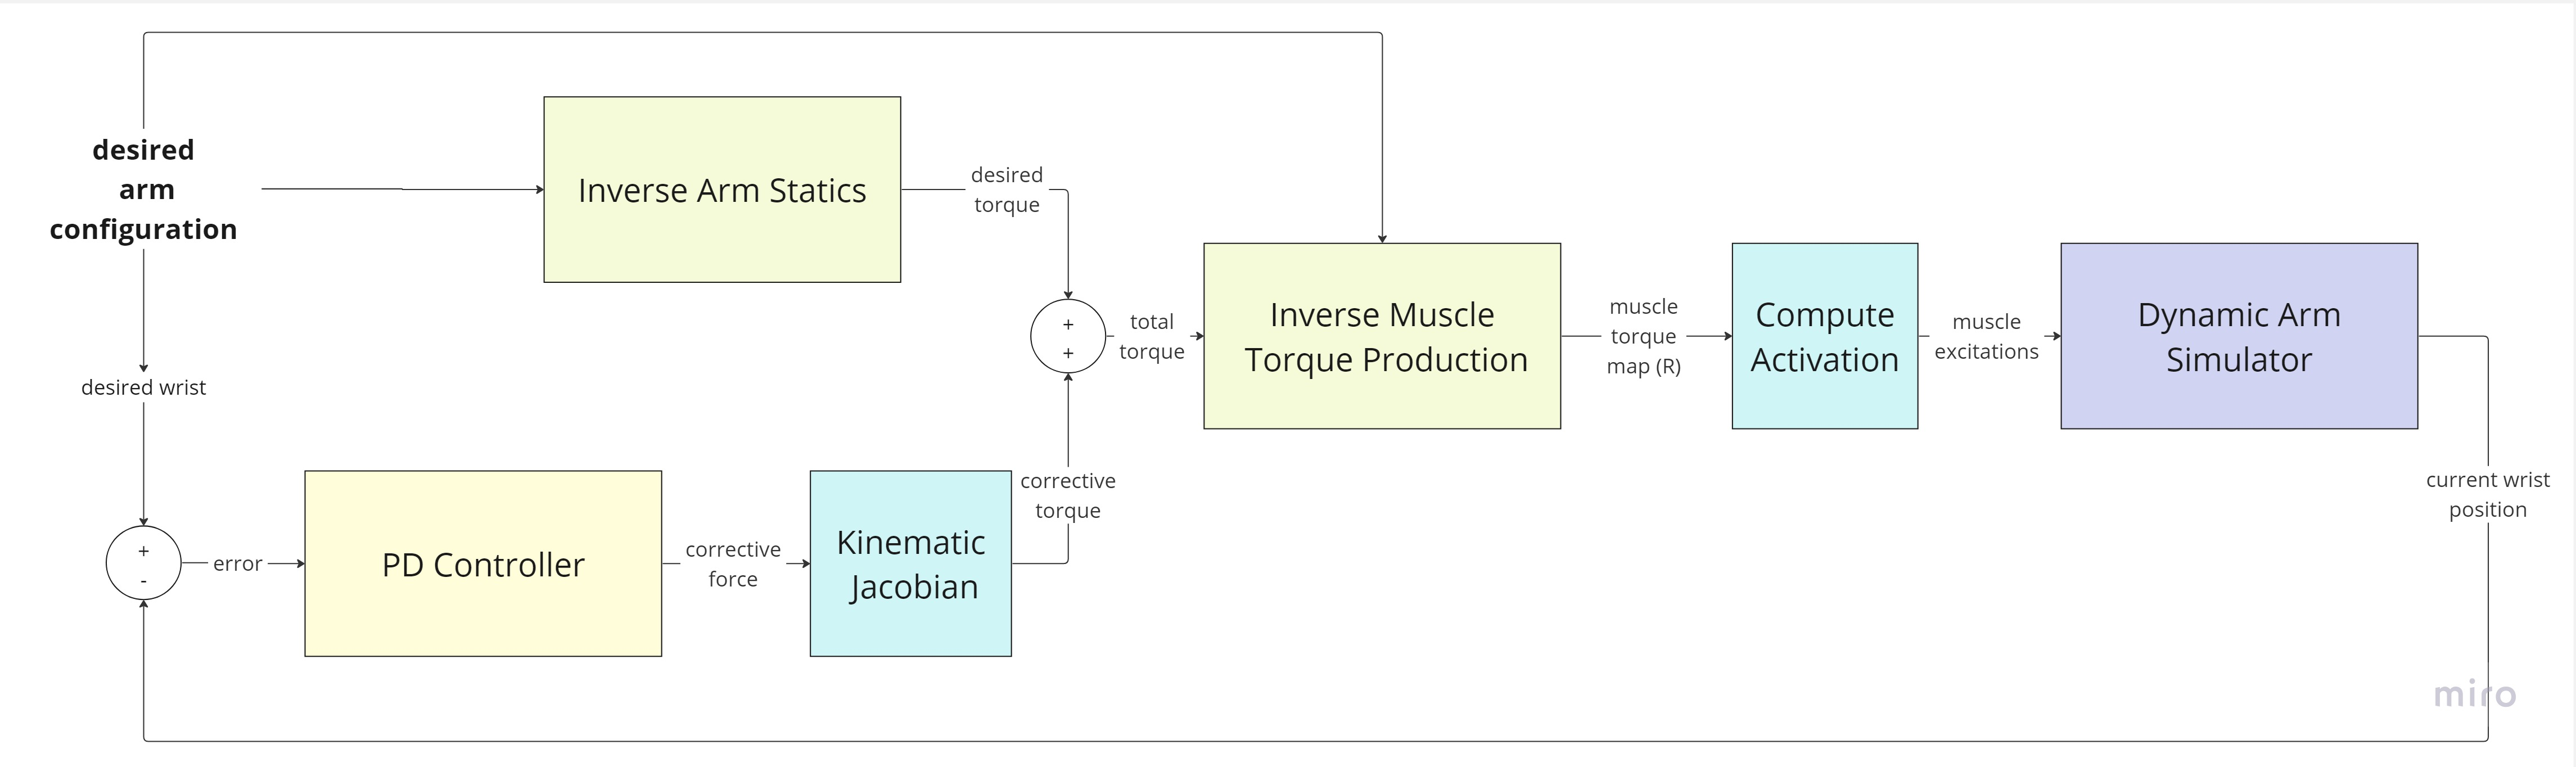
\includegraphics[width=1\textwidth]{Pictures/Controller/controller-diagram.jpg}
    \caption{Controller Block Diagram inspired in \cite{QSC}}
    \label{fig:BDC}
\end{figure}

To assure the PID Controller's performance, an exhaustive tuning was undertaken across 20 different positions, concluding in values of \(K_p = 300\) and \(K_i = 100\). 

With this tuned controller, a grid, encompassing 960 points, was generated using the \textbf{create\_grid} function (refer to Section \ref{sec:tp}). Each point's arm configuration was calculated using the PI force controller, as detailed in Section \ref{sec:PI}. The feasibility of a point was determined by the ability of the controller to sustain for 1 second its position with an error margin of 0.1. For clarification purposes, the start and the goal position of the controller are set to be the same. 
For seamless and accurate operations, a time step (\(t_{step}\)) of 0.001 is employed. To improve the controller's stability an auxiliary force is exerted on the arm in the first 100 steps. This eliminates potential oscillations and assures a better control performance.

The figures below present the generated grid. Points in red signify positions where the controller failed to find the neural excitation needed to sustain for 1 second. In contrast, green points indicate successful stabilization by the controller. These feasible points will be used in the following section (Section \ref{sec:path}) to generate paths for the arm to follow. 

\subsection{PID Tuning}
\newpage
\section{Path Following Quasi-Static Control Development } \label{sec:path}

The goal is to develop a controller that allows the dynamic arm  to navigate or follow a specific trajectory or path. This will simulate the rehabilitation reaching task to be performed. For more information on rehabilitation tasks refer back to Section \ref{rehabilitation_task}. Quasi-static control allows to design a safe, precise and movement-controlled therapy, as it focuses on slow, steady and controlled operations. It facilitates the decomposition of the entire reaching path trajectory into smaller static positions. Dividing the task into smaller steps offers some benefits under the rehabilitation lens:
\begin{itemize}
    \item \textbf{Gradual Progression}. Rehabilitation often demands gradual approach towards exercises, specially for recovering patients. progress.
    \item \textbf{Progress Tracking} Breaking the movement into smaller steps helps not only patients to progress at a comfortable and safe pace but allows to keep track of the progress.
    \item \textbf{Minimized Fatigue} Continuous motions can take a toll in patients with limited strength and endurance. Smaller tasks reduce muscle and join strain preventing fatigue. Using a quasi-static controller can help modify the parameters to adjust to the patient's abilities. 
\end{itemize}

For a clearer understanding of the quasi-static control designed, refer to the flow diagram included in this chapter (Figure \ref{fig:PathController}). Here’s a descriptive step-by-step breakdown of the process of path controller:

\begin{enumerate}
    \item \textbf{Selection of Target Position}: From a set of feasible points, a target position is chosen. This serves as the end-point or goal for the system.
    
    \item \textbf{Path Discovery via the 'find path' Function}: The selected target position is input into the 'find path' function. This function works by first identifying the nearest neighbors from the feasible points workspace. Among the first 200 nearest neighbors of the starting point, it selects one that:
    \begin{itemize}
        \item Is at a distance \(d = 4\) units away from the starting point. This distance recommendation comes from the paper \cite{QSC}.
        \item Lies in the direction of the end-point or target position.
    \end{itemize}
    Through this method, a path consisting of multiple positions is generated.
    
    \item \textbf{Setting Initial Simulation Parameters}: At the beginning of the simulation, the initial position from the path is defined. Moreover the simulation parameter are set: \(t_{step} = 0.003\), and a $frequency$ of 30Hz. The variable $frequency$ refers to the rate at which the FES (Functional Electrical Stimulation) device can change its input. This is a criteria detailed on the design Section \ref{Design} limited by the FES devices.
    
    \item \textbf{Control Loop}: The control loop operates as previously outlined in the Section \ref{NeuralController} , with a few distinct modifications:
    \begin{itemize}
        \item \textbf{Neural Excitation}: This only takes place at set intervals based on the defined $frequency$.
        \item \textbf{Position Switching}: At every $time_{switch}$ the position in the control system is updated to the subsequent one in the predefined path array.
        
        If the hand has not reached the vicinity of the targeted position within the set time frame of $time_{switch}$, the system will attempt to reach the position a maximum of two more times before potentially moving to the next point or terminating.
    \end{itemize}
\end{enumerate}

In conclusion, the proposed controller is designed to guide a dynamic arm through specified trajectories, mimicking the rehabilitation reaching tasks outlined in Section \ref{rehabilitation_task}. Quasi-static control is used to emphasize safety, precision and control, three key components for a successful rehabilitation. Key components of the control system presented include a \textbf{\textit{find\_path} }function that uses KNN to find the best positions that will define the path to the desired target. Moreover the control loop, adapted from the one on Section \ref{NeuralController}, operated with timed neural excitation (controlled by the variable $frequency$) and position switching to guide the arm accurately along the predefined path (controlled by variable $time_{switch}$).



\begin{figure}[h!]
    \centering
    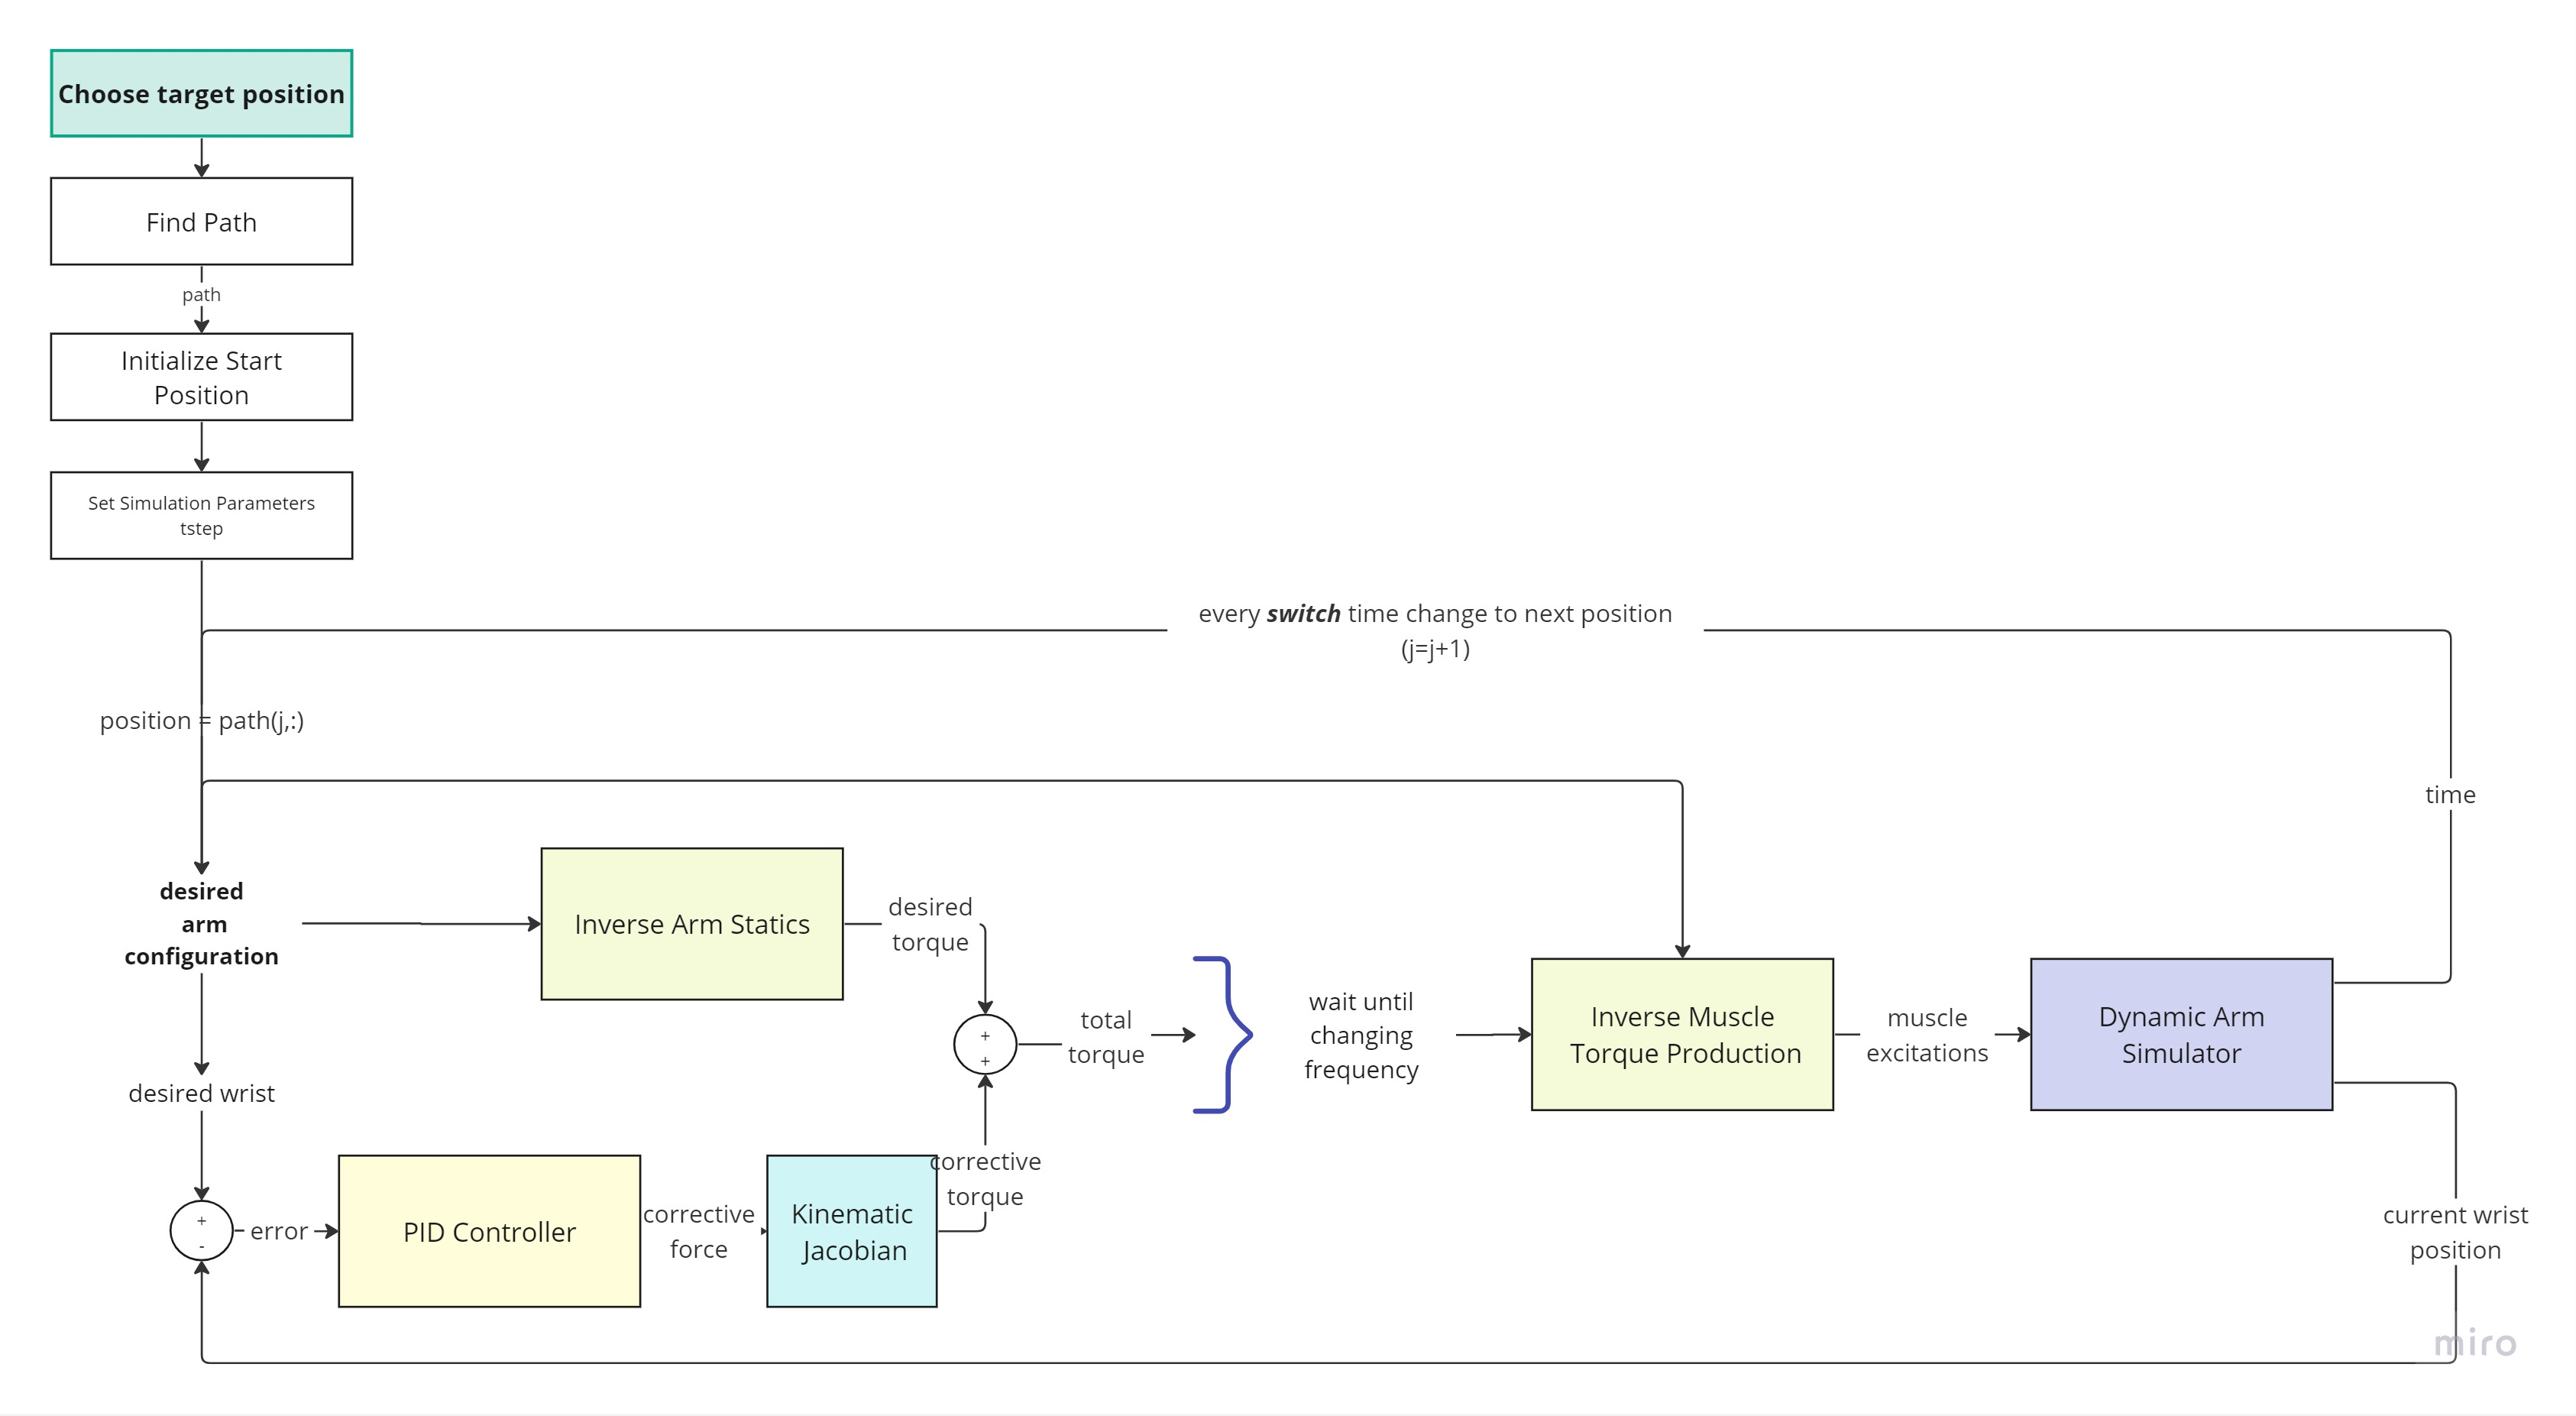
\includegraphics[width=1\textwidth]{Pictures/Controller/Quasi-Static Path Controller.jpg}
    \caption{Flow Diagram Quasi-Static Path Controller }
    \label{fig:PathController}
\end{figure}

\newpage
\section{EMG-Influenced Control Development}

\newpage
\begin{landscape} % Start landscape page
  \begin{figure}[h!]
    \centering
    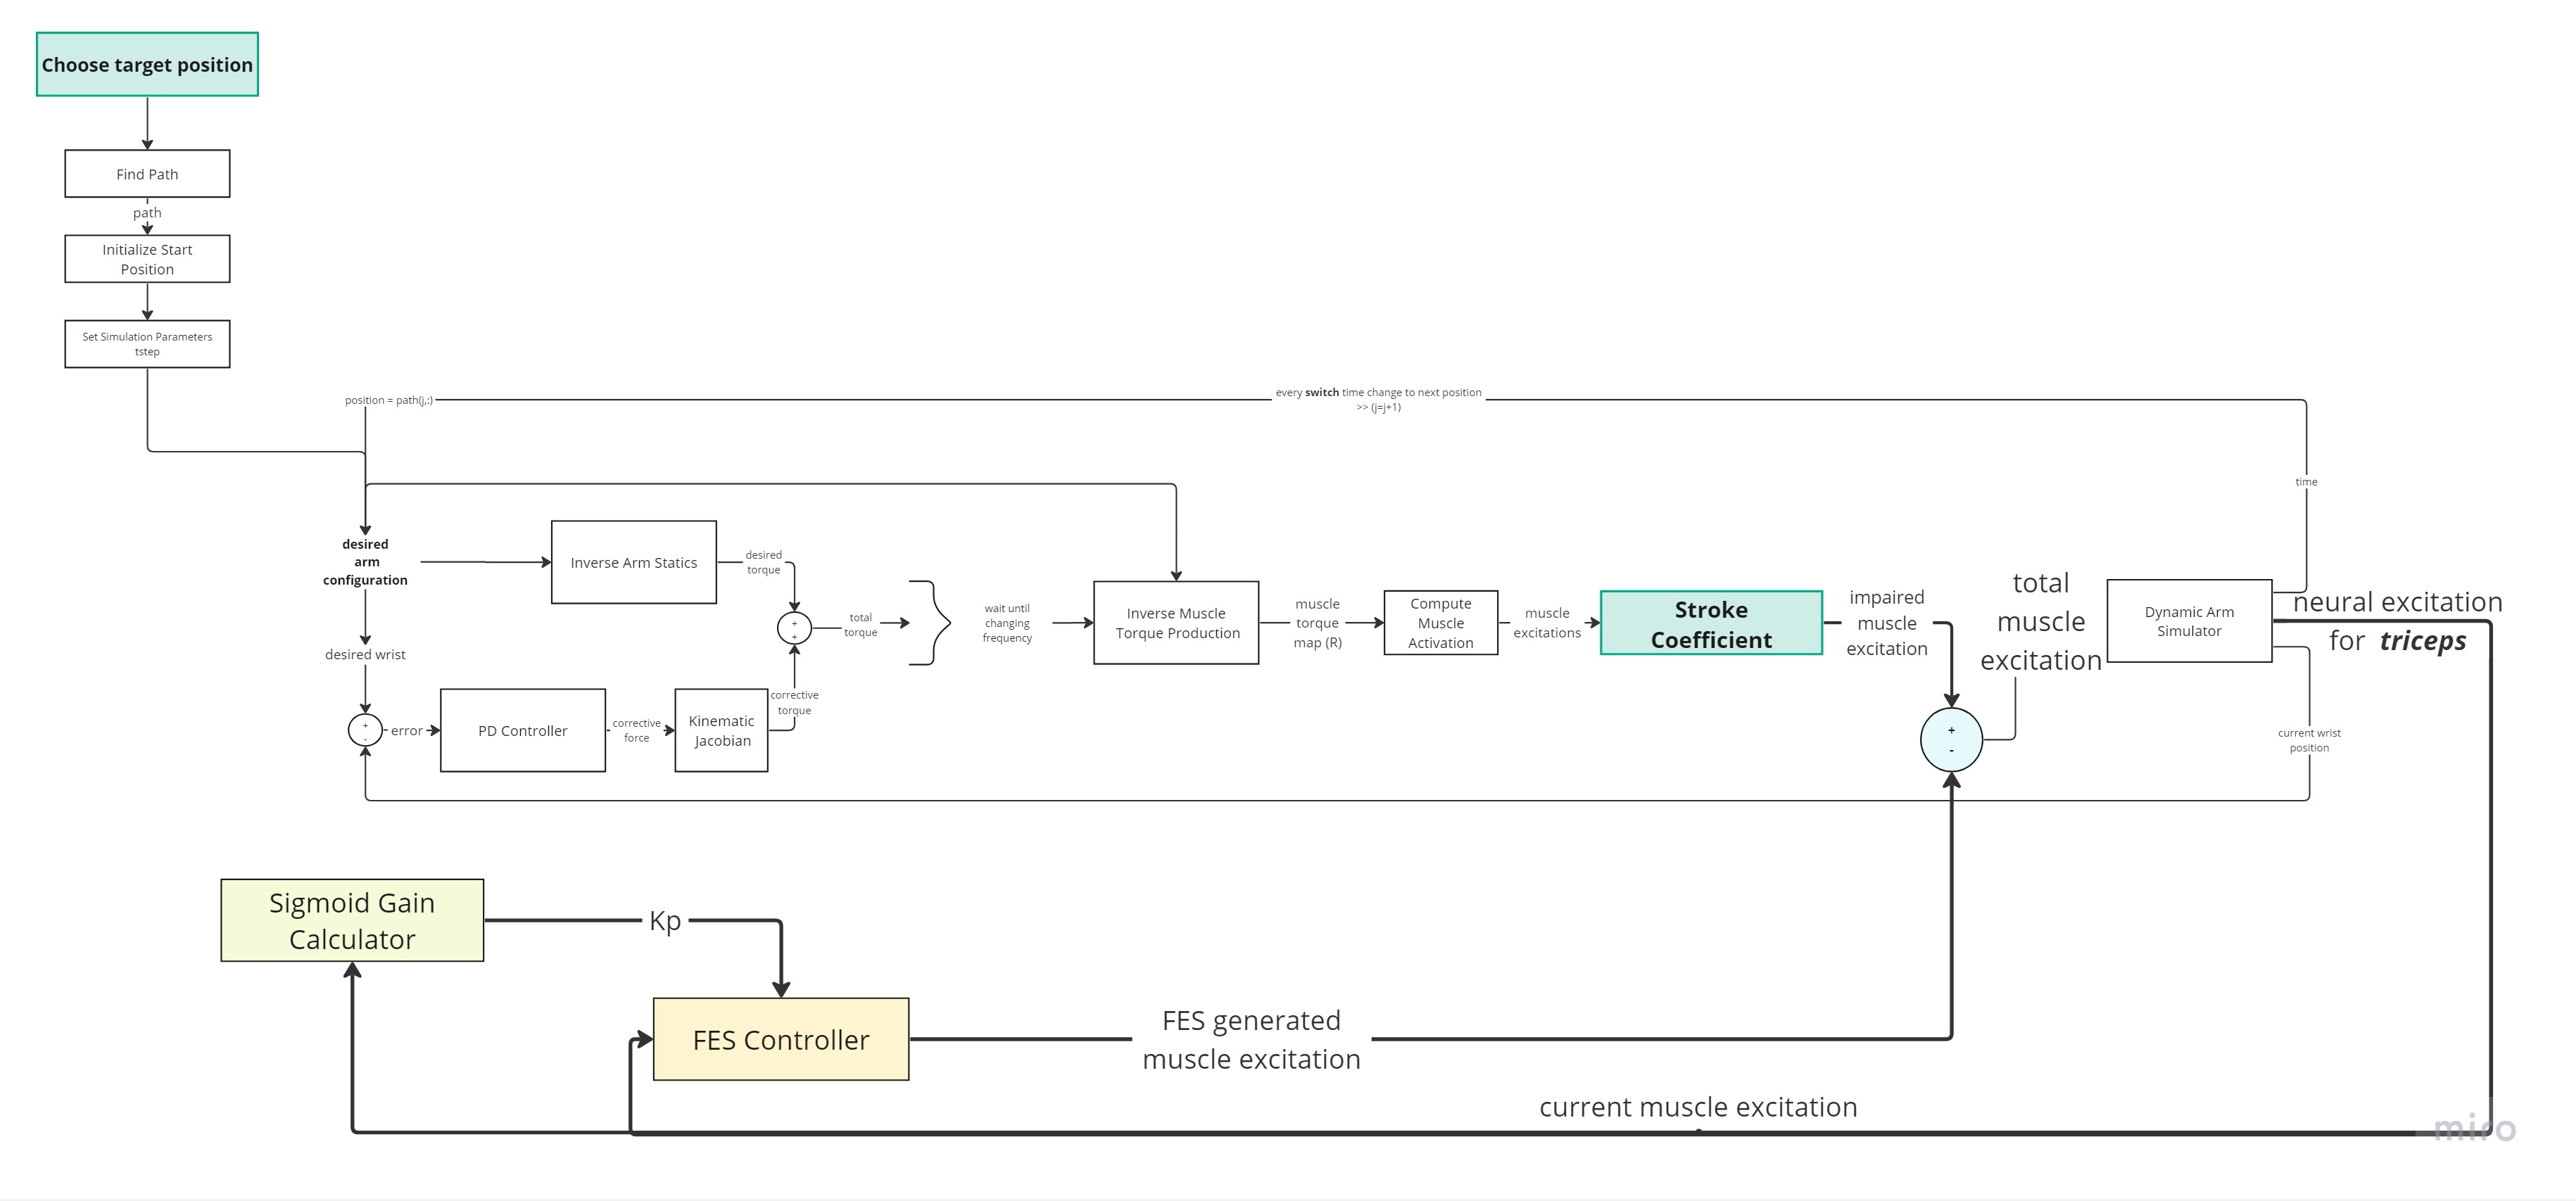
\includegraphics[width=1.7\textwidth]{Pictures/Controller/FESController.jpg} % Replace "filename.jpg" with the name of your image file
    \caption{Flow Diagram for EMG-influenced FES Controller} % Optional caption
    \label{fig:FESController} % Optional label for referencing
  \end{figure}
\end{landscape} % End landscape page

